\chapter{Conclusions} \label{ch:conclusion}

% Main points:
% - What has been accomplished that was not there before
% - What is the most relevant follow up work
% - What are the most relevant challenges
% - Make sure to connect with the introduction, that is refer to the problems presented there and the degree to wich they are addressed.


% 1. Accomplishments (Separate technical and scientific?)
% - Use of system level models
% - Develop multi-objective optimzation formualtions and solution techniques, with the primary aim of modular design, but applicable to many design and analysis situtations were multiple conflicting objectives exist -> for example?
% - ...
% - (reference to the arrow figure)

Despite the high interst in the application of modular design in synthetic biology and related fields,
%and more specifically platform strain design in metabolic engineering, are important topics in the field, however
not many quantiative and systematic design framworks exist.
This thesis has developed such tools, notably using multi-objective optimization as basis to formulate modular design problems in synthetic biology.
The driving application behind these developments is whole-cell biocatalysis, a technology that can lead to renewable and efficient manufacturing of chemicals, fuels, and materials.
%multi-objective optimization opens many new possibilites for more realistic design simulations ...
%As a driving application of this method, particular atention has been paid to biocatalysis.
%applications,
Primarily guided by their intuition, researchers at companies and universities have built platform strains that recycle the knowledge and labor applied towards a given product to expand towards other molecules that use similar metabolic pathways. %TODO: "guided by their intuition" might sound pretentious or not even very clear
Motivated by this principle, several iterations of the ModCell design method have been developed and applied to elucidate modular design principles for biocatalytic strains (Figure~\ref{fig8:arrow}).
%Additionally, tools have been developed to characterized expected module behavior (compatibility) and key areas of core chassis metabolism (interfaces) that are critical for correct module operation.
Overall, this effort contributes to the current wave of converting molecular biology into a more quantitative science by developing and applying mechanistic models of metabolism, and provides new tools to develop modular biocatalytic strains.
We envision these new design tools will lower the cost and time required to develop efficient an robust biocatalytic strains that harness the large space of molecules resulting from natural and synthetic metabolic pathways.
% "Recently, modular cell engineering has been proposed as an innovative approach to accelerate strain engineering process, harnessing a large space of molecules derived from rich and diverse cellular metabolism and thus pushing whole-cell biocatalysis towards an industrially competitive technology \citep{trinh2016}."
% In addition to bioca

\begin{figure}[h]
  \centering
  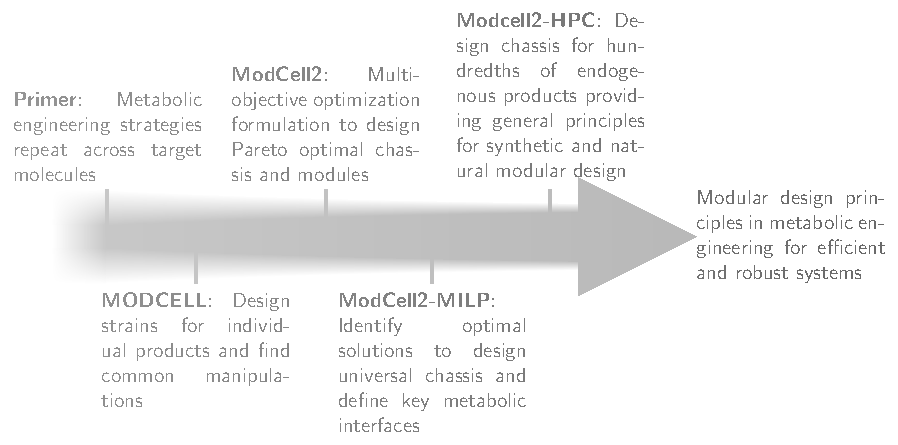
\includegraphics[width=\textwidth]{timeline-arrow}
    \caption{Advances of this thesis.}
    \label{fig8:arrow}
\end{figure}


% 2. Next wave: The need of the problem framing to build and study strains in this context
% - While techniques have general application,  Predictions without validation is only part of the story.
% - There are two views: 1)design simulation to build; 2)Use simulation to contextualize
% - Modcell falls in case 1. The problem formulation requires that experimental data is ... this was as much as possible done by examining the literature, primarly in the field of metabolic engineering, where genetic manipulations are implemented and characterized ...
% - C therm chapter is case 2.
% - Next wave -> build and characterize

% TODO: The main point does not stand out, and the begining of the paragraph feels confusing
In computational biology, algorithmic and modeling challenges are critical aspects, however, as an applied field, simulation efforts need to be connected to experimental ones.
Briding the gap between simulations and experiments, can be addressed from two perspectives:
%As a computional biologist, ... this is often addressed with two framings:
i) Simulations are used a priori to generate a hypothesis, then experiments are conducted to test the hypothesis and also perhaps to validate the accuracy of the simulation;
ii) Experimental observations are available, and simulations are used to explain them, i.e., to assist in developing a scientific theory.
Chapter~\ref{ch:ctherm} falls under the second category, where the developed metabolic model is used to explain proteomics data at the system level to contribute towards a redox-imbalance theory of biocatalytic \textit{C. thermocellum} strains. % NOTE: Don't be too specific here
However, the majority of this work, formulated as a biocatalysis strain design problem, falls under the first category.
Hence, the next wave of development of modular cell design principles should be focused on the implementation and characterization of the strains proposed here, closing the design-build-test cycle.

%post hoc addition of experimental data %Watch out since post hoc, can have quite negative connotations %Watch out since post hoc, can have quite negative connotations


% 3. Future perspective (be general and tie back to the **intro**)
% - Main challenges in the relevant fields
% - highly predictive does not seem around the corner
% - time horizon for application
% - Ethical concerns: Increased inequality and existential risk

As with most contemporary scientific works, this thesis contributes a drop to the ocean of knowledge needed to address the scientific and social challenges of our time.
%Scientific and social challenges,
 %my grain of sand in building and using cellular models built from first principles to .... As well as devel... that...
 There are multiple relevant facets to the problems tackled here. In particular, biological modeling remains limited by our ability to integrate disparate data types, and the technical challenges of measuring certain parameters such as the catalytic efficency of each enzyme;  while biocatalysis remains limited by poor enzyme expression and function in pathways of interest. %our ability to genetically engineer pathways that are efficient and hence can carry sufficient metabolic flux for the titers, productivity and yields, required for industrial application. % TODO: Too general, need to define the challenge more precisely. THe key challenge is that enzymes express poorly
%In the field of artificial intelligence, the ability to build an artificial general intelligence (i.e., comparable to human intelligence) does not seem to be around the corner. % TODO: Add citation, this might seem ranty/ why is the analogy relevant?
%Similarly
Overall, our ability to build and manipulate living organisms for any feasible biological function, does not seem to be around the corner.
% TODO: due to what? due to the lack of both essential information and models that integrate the information.
However, the key challenges needed for successful applied technologies are rapidly being overcome, as evidenced by the many biotechnology companies emerging over the last decade.
As we develop novel technologies, we must also become aware of the ethical and existential risks associated with them.
For example, genetic engineering for enhanced cognitive abilities could likely become an expensive medical treatment that increases the wealth gap in society. % (similar ideas are explored in the film gattacca)
These concerns are specially relevant for the field of synthetic biology, as genetic engineering tools becomes more widely available enabling DIY biohacking \citep{bennett2009}.
These developments could pose an existential risk for our current civilization given that a highly desctructive technology becomes suffiently easy to use,  and such technology cannot be ``uninvented" or effectively policed.
This challenge can be illustrated through The Urn of Inventions metaphore (Figure~\ref{fig8:vwh}) \citep{bostrom2019}. % NOTE: Follow up this sentence to expl
% NOTE: Make sure this feels "complete" but that further reading is available to expand, do not lean on citations. It has to make sense entirely in this context.
% NOTE: Last sentence needs to be conclusive
Briefly, consider technologies to be balls in an urn, and our current strategy is to draw balls as fast as possible, perhaps to obtain wealth, prestige, and citations. However, if there was a ``black ball" technology, which discovery would have highly damaging consequences, alternative strategies should be considered to prevent a global catstrophe.
In summary, while issues like climate change already receive considerable attention, we should become more aware of other dangers of technological development and create policies accordingly.

% Important paper
% https://www.nature.com/articles/nbt1209-1109
%More immediatly concerning, is the increasing availability of gene synthesis and genetic engineering tools.

% Key paper to cite:
% https://onlinelibrary.wiley.com/doi/full/10.1111/1758-5899.12718
%
%"Similarly, cheaply available genetic engineering tools could enable the development of pandemic organisms with very few resources.

%Nick Bostrom presents this problem with the "urn of inventions" metaphor, where each new technology is a ball that can be drawn, and among the balls there are some black balls that represent threating technologies.
%Our current strategy is to draw balls from the urn as fast as possible, and hope that we do not draw a black ball.
%Some areas, such as synthetic biology, could produce a discovery that suddenly democratizes mass destruction, e.g. by empowering individuals to kill hundreds of millions of people using readily available materials. In order for civilization to have a general capacity to deal with “black ball” inventions of this type, it would need a system of ubiquitous real‐time worldwide surveillance. In some scenarios, such a system would need to be in place before the technology is invented."
%

\begin{figure}[h]
  \centering
  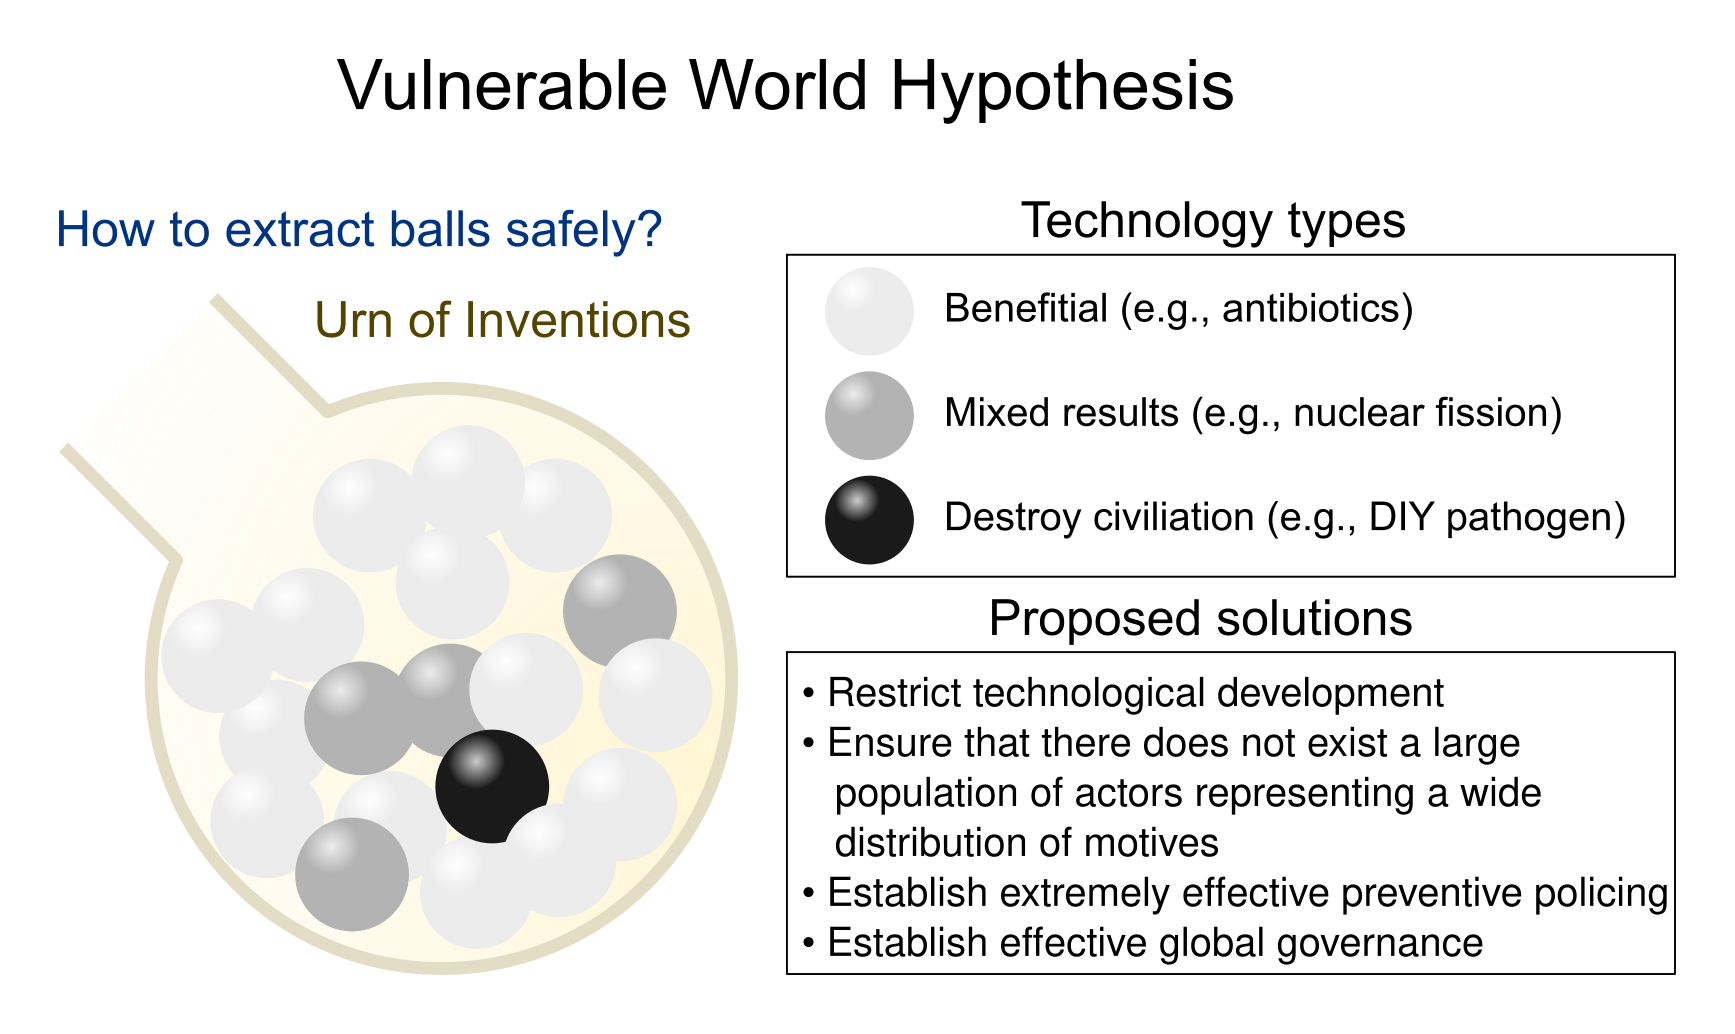
\includegraphics[width=\textwidth]{urn-of-inventions}
    \caption[The Vulnerable World Hypothesis]{The Vulnerable World Hypothesis described through the Urn of Inventions metaphor. The hypothesis is that there exists a technology that once discovered would have devastating effects to civiliation. If the hypothesis is true, we should reconsider how scientific discovery is to be conducted to minimize such risk. See \citep{bostrom2019} for further explanation of the topic and proposed solutions.}
    \label{fig8:vwh}
\end{figure}
